\documentclass{template/openetcs_report}
% Use the option "nocc" if the document is not licensed under Creative Commons
%\documentclass[nocc]{template/openetcs_article}
\usepackage{lipsum,url}
\usepackage{supertabular}
\usepackage{multirow}
\usepackage{color, colortbl}
\definecolor{gray}{rgb}{0.8,0.8,0.8}
\usepackage[modulo]{lineno}
\graphicspath{{./template/}{.}{./images/}}

\begin{document}
\frontmatter
\project{openETCS}

%Please do not change anything above this line
%============================
% The document metadata is defined below

%assign a report number here
\reportnum{OETCS/WP2/?}

%define your workpackage here
\wp{Work-Package 2}

%set a title here
\title{Scrum Prozess ETCS}

%set a subtitle here
\subtitle{}

%set the date of the report here
\date{August 2015} % \\ Revised April 2015}

%document approval
%define the name and affiliation of the people involved in the documents approbation here
\creatorname{Abdelnasir Mohamed}
\creatoraffil{AEbt}

\techassessorname{}
\techassessoraffil{}

\qualityassessorname{}
\qualityassessoraffil{}

\approvalname{Klaus-R\"udiger Hase}
\approvalaffil{DB Netz}

%define a list of authors and their affiliation here

\author{Abdelnasir Mohamed}

\affiliation{AEbt Angewandte Eisenbahntechnik GmbH\\
  Adam-Klein-Str. 26 \\
  90429 Nürnberg, Germany\\
  eMail: abdelnasir.mohamed@aebt.de \\
  WebSite: www.aebt.de}  

\author{Jan Welte}

\affiliation{Technische Universität Braunschweig\\
  Institute for Traffic Safety and Automation Engineering\\
  Hermann-Blenk-Str. 42\\
  38108 Braunschweig, Germany\\
  eMail: openetcs@iva.ing.tu-bs.de \\
  WebSite: www.iva.ing.tu-bs.de}
  

%add yourself as author, if you contributed to the document



% define the coverart
\coverart[width=350pt]{openETCS_EUPL}

%define the type of report
\reporttype{Output Document}


\begin{abstract}

\end{abstract}

%=============================
%Do not change the next three lines
\maketitle
\tableofcontents
\listoffiguresandtables
\newpage
%=============================

\chapter{Document Control}

\begin{tabular}{|p{4.4cm}|p{8.7cm}|}
\hline
\multicolumn{2}{|c|}{Document information} \\
\hline
Work Package &    \\
Deliverable ID & \\
\hline
Document title & openETCS \\
Document version & 01.1 \\
Document authors (org.)  & Jan Welte (TU-BS) and Abdelnasir Mohamed (AEbt)\\
\hline
\end{tabular}

\begin{tabular}{|p{4.4cm}|p{8.7cm}|}
\hline
\multicolumn{2}{|c|}{Review information} \\
\hline
Last version reviewed & 0.1 \\
\hline
Main reviewers (org.) & \\
\hline
\end{tabular}

\begin{tabular}{|p{2.2cm}|p{4cm}|p{4cm}|p{2cm}|}
\hline
\multicolumn{4}{|c|}{Approbation} \\
\hline
  &  Name & Role & Date   \\
\hline  
Written by    &  Jan Welte & WP4-T4.4 Task Leader  &  March 2015\\
\hline
Approved by & -- & -- & \\
\hline
\end{tabular}

\begin{tabular}{|p{2.2cm}|p{2cm}|p{3cm}|p{5cm}|}
\hline
\multicolumn{4}{|c|}{Document evolution} \\
\hline
Version &  Date & Author(s) & Justification  \\
\hline
0.1 & 18/08/2015 & Jan Welte &  Document creation \\
\hline  
00.1 & 28/01/2014 &  &   \\

\hline  
\end{tabular}
\newpage

% The actual document starts below this line
%=============================

\mainmatter

\chapter{Introduction}
\label{sec:introduction}

Nasir

Short introduction to this document.

\begin{itemize}
\item extension to QA-Plan and Process Description
\end{itemize}

\section{Purpose}
\label{sec:purpose}

Nasir

purpose of this document

\begin{itemize}
\item showing principals of the iterative work in openETCS development life cycle 
\item explaining agile principles to coordinate work and complete artifacts
\end{itemize}

%\section{Document Structure}
%\label{sec:document-structure}



%\section{Document Evolution}



\section{Reference Documents}
\label{sec:refdoc}

This document essentially refers to the following standards, ETCS specification documents and openETCS project documents.

\begin{itemize}
\item \textbf{ISO~9000} --- 12/2005 --- \emph{Quality management}
\item \textbf{ISO~9001} --- 12/2008 --- \emph{Quality management systems — Requirements}
\item \textbf{ISO~25010} --- 03/2011 --- \emph{Systems and software engineering -- Systems and software Quality Requirements and Evaluation (SQuaRE) -- System and software quality models}
\item \textbf{CENELEC EN~50126-1} --- 01/2000 --- \emph{Railways applications –- The specification and 
demonstration of Reliability, Availability, Maintenability and Safety (RAMS) –- Part 1: 
Basic requirements and generic process}
\item \textbf{CENELEC EN~50128} --- 10/2011 --- \emph{Railway applications -- Communication, signalling and 
processing systems -- Software for railway control and protection systems}
\item \textbf{CENELEC EN~50129} --- 05/2003 --- \emph{Railway applications –- Communication, signalling and 
processing systems –- Safety related electronic systems for signalling}
\item \textbf{CCS~TSI} --- \emph{ CCS TSI for HS and CR transeuropean rail has been adopted by a Commission Decision 2012/88/EU on the 25th January 2012}
\item \textbf{SUBSET-026} 3.3.0 --- \emph{System Requirement Specification}
\item \textbf{SUBSET-091} 3.2.0 --- \emph{Safety Requirements for the Technical Interoperability
of ETCS in Levels 1 \& 2}
\item \textbf{SUBSET-088} 2.3.0 --- \emph{ETCS Application Levels 1 \& 2 - Safety Analysis}
\item \textbf{OpenETCS FPP} --- \emph{Project Outline Full Project Proposal Annex OpenETCS} -- v2.2
\item \textbf{OpenETCS D2.2} -- Report on CENELEC standard
\item \textbf{OpenETCS D2.3} -- Definition of the overall process for the formal description of ETCS and the rail system it works in 
\item \textbf{OpenETCS D2.4} -- Definition of the methods used to perform the formal description
\end{itemize}


%%%%%%%%%%%%%%%%%%%%%%%%%%%%%%%%%%%%%%%%%%%%%%%%%%%%%%%%%%%%%%%

\section{Glossary}
\label{sec:glossary}



\begin{tabular}{rl}
\textbf{ACedit} & Assurance Case Editor \\ 
\textbf{ARM} & Argumentation  Metamodel \\ 
\textbf{ETCS} & European Train Control System \\ \textbf{ERA} & European Railway Agency \\ \textbf{FMEA} & Failure Mode Effect Analysis \\ 
\textbf{GSN} & Goal Structured Notation \\ 
\textbf{MoRC} & Management of Radio Communication \\ 
\textbf{RAMS} & Reliability, Availability, Maintainability and Safety \\
\textbf{SIL} & Safety Integrity Level \\ 
\textbf{SRS} & System Requirement Specification \\ 
\textbf{THR} & Tolerable Hazard Rate \\ 
\textbf{V\&V} & Verification \& Validation \\ 
\end{tabular} 




\section{Background Information}
\label{sec:Background}


\subsection{Agile Development}

Jan

really short introduction to the concept of agile development overall

\subsection{Scrum}

Nasir

introduction to Scrum 

based on text in QA-Plan as it fits
\begin{itemize}
\item Concept of Scrum
\item Roles
\item Scrum Process
\end{itemize}


\chapter{Agile Development in OpenETCS}
\label{sec:agile}

Jan

Basic concept of agile development in openETCS.
Allocation of agile work principles to 

\begin{itemize}
\item allocating agile work activities to the iterative work in openETCS development life cycle (phases nd artifacts) 
\item describe overlap between EN 50128 roles and Scrum roles
\end{itemize}


\chapter{Scrum of Scrum}
\label{sec:Scrumofscrum}

Nasir

Short introduction to principle of splitting work between different teams, as required by the EN 50128

Principles of grooming work and filling backlogs for distributed Scrum Teams by dynamic work allocation.

Text based on wiki page by Marc Behrens

\textit{Objective:} Ongoing verification and validation of openETCS development artifacts are performed within the framework of openETCS scrum process. This page describes the interface of agile verification and validation to the top level customer as well as the scrum process within the verification and validation itself.

\begin{figure}[h]
\centering
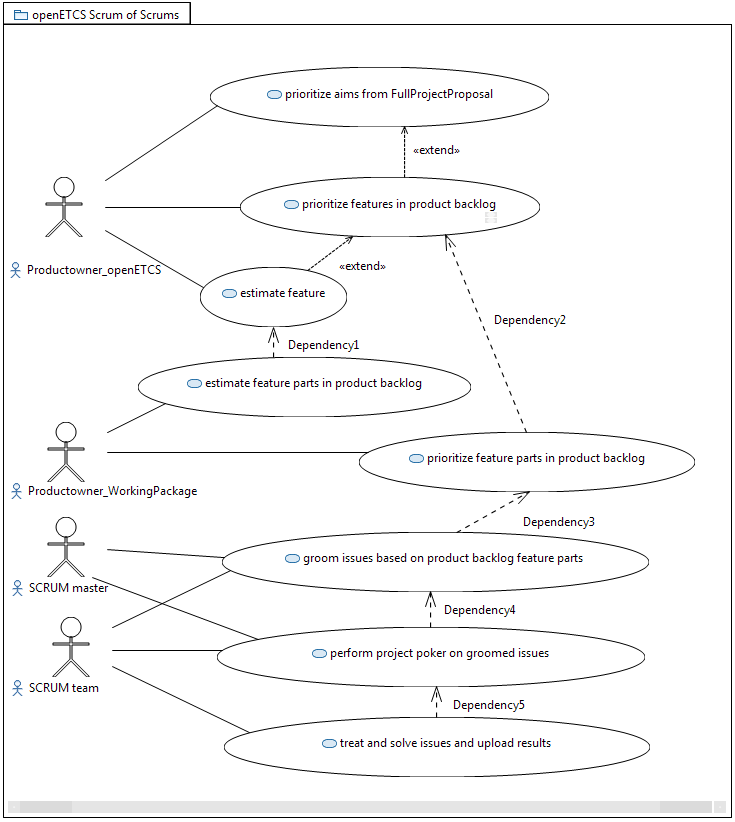
\includegraphics[width=0.7\linewidth]{./images/openETCSVnVScrumOfScrum_02}
\caption{openETCS scrum of scrums}
\label{fig:openETCSVnVScrumOfScrum}
\end{figure}

Within the agile scrum process of openETCS different backlogs are used to synchronise the top level project goals with the tasks performed within the project: 

\begin{itemize}
\item Each backlog itself consists of items which are represented within the github issue tracker. 
\item For each backlog a Product Owner is assigned to coordinate and prioritize the items.
\item Each Story Point (SP) is estimated to be worth one person day.
\end{itemize}


\textbf{The Product Backlog (Product Owner: Klaus-Rüdiger Hase)}
The Product Backlog consists of top level \textit{Features} by which the product is described.
\begin{itemize}
\item  Each Feature itself is estimated by the product owner on how many Story Points this Feature is worth.
\item  A Feature itself is divided into **Feature Parts**.
\item  A Feature Part is related directly to a working package and the repository the work is documented in.
\item  Each Feature Part itself is estimated and prioritized by the product owner on how many Story Points this Feature Part is worth.
\end{itemize}


By estimating the feature the feature becomes accepted on product Level.
The Product Backlog is maintained during a regular meeting.

\textbf{Transferring the Features from the \textit{Product Backlog} to the Verification and Validation Sprint Backlog}
During regular grooming sessions the scrum team extracts the items with highest priority out of the Product Backlog and refines them to issues within the repository mentioned within the Feature Part.
On these issues Project Poker is performed on and by this Story Points are assigned. The decision on which items enter the Sprint Backlog is based on the maximum benefit analysis taking into account the priority as well as the story points.

\textbf{Sprint Backlog}
The \textit{Sprint Backlog} consists of issues which are processed during the sprint.
During the sprint the success is tracked against the Sprint Backlog.
The Story Points are earned once the complete result of what has been groomed is uploaded to the github.

\chapter{Release Principals}
\label{sec:Releases}

Jan

principles of artifact releases (specially models) and their verification and validation
configuration management of design artifacts, test specifications and test reports
change management via issues, status of documents, criteria for releases and assessment


\chapter{Conclusion}
\label{sec:conclusion}

can be left open for now

final conclusion of content 


%\bibliographystyle{unsrt} %
%\bibliography{./ref/ref-HaRA}


%===================================================
%Do NOT change anything below this line

\end{document}


